\ifx\inkludert\undefined
\input{preamble}
\usepackage{xr}
\externaldocument{lin-alg}
\newcommand{\kapittel}[2]{\setcounter{chapter}{#1}\addtocounter{chapter}{-1}\chapter{#2}}
\newcommand{\kapittelslutt}{\enddocument}
\begin{document}
\chapterstyle{tma4110}
\pagestyle{plain}
\fi


\kapittel{10}{Komplekse tall}
\label{ch:komplekse-tall}


Oppfinnelsen av nye tallsystemer henger gjerne sammen med polynomligninger. Ligningen 
\[
2x+4=0
\]
har ingen positiv løsning, selv om koeffisientene er positive tall. 
Vi må altså inn med negative tall, og skrive 
\[
x=-2.
\]
Ligningen
\[
2x-3=0
\]
har ingen heltallig løsning, selv om koeffisientente er hele tall, så nå må vi inn med rasjonale tall:
\[
x=\frac{3}{2}
\]
Ligningen
\[
x^2-2=0
\]
har ingen rasjonale løsninger, siden
\[
x=\sqrt{2}
\]
ikke kan skrives som en brøk. Dette viste vi i TMA4100, før lunsj på fredag i uke 33. 
Generelt er det slik at en polynomlikning
\[
a_nx^n+a_{n-1}x^{n-1}+...+a_1x+a_0=0
\]
ikke nødvendigvis har en løsning i det tallsystemet koeffisientene er hentet fra. 
Man kan spørre seg hvorvidt det finnes tallsystemer der en vilkårlig polynomlikning alltid har løsning, 
og svaret er ja. 
Vi skal ta for oss et slikt tallsystem, nemlig de \defterm{komplekse tallene}.
%Likningen 
%\[
%x^2+1=0
%\]
%ingen reelle løsninger. Hva gjør vi med det?


\section*{Den imaginære enheten}
Ligningen
\[
x^2+1=0
\]
har ingen reell løsning. 
La oss finne opp et nytt tall. Vi kaller det $i$, den \emph{den imaginære enheten}. 
Nå kan det være fristende å løse likningen over for $x$, definere
\[
i=\sqrt{-1},
\]
og så skrive kvadratroten av negative tall på en pen måte:
\begin{equation*}
\sqrt{-4}=\sqrt{4\cdot (-1)}=\sqrt{4}\cdot \sqrt{(-1)}=2i.
\end{equation*}
Dette må man være litt forsiktig med, 
for vanlige regneregler for røtter gjelder ikke for negative tall:
\begin{align*}
1&=(-1)\cdot(-1)\\&=\sqrt{(-1)\cdot (-1)}\\&=\sqrt{-1}\cdot \sqrt{ -1}=i^2=-1.
\end{align*}
Men disse suspekte beregningene gir oss allikevel en pekepinn om hva vi ønsker å oppnå. 
En bedre løsning er å definere $i$ ved ligningen
\[
i^2=-1,
\]
og så får vi være enige om å si $2i$ istedet for $\sqrt{-4}$, 
og skulle vi slumpe til å ta roten av negative tall, 
må vi passe på at vi ikke gjør noe som ikke er riktig.

Løser vi likningen
\[
x^2+x+1=0
\]
gir annengradsformelen
\[
x=\frac{-b\pm\sqrt{b^2-4ac}}{2a}
\]
at
\[
x=\frac{-1\pm\sqrt{-3}}{2}=-\frac{1}{2}\pm\frac{\sqrt{3}}{2}i,
\]
og dette inspirerer oss til å definere \emph{komplekse tall} som 
\[
z=a+bi.
\]
Her er $a$ og $b$ reelle tall. 
De kalles henholdsvis \emph{realdelen} og \emph{imaginærdelen} til $z$,
og skrives gjerne $\Re z$ og $\Im z$. 
Mengden av alle komplekse tall kalles $\C$. 
Dersom $b=0$, er $z$ reell, og vi ser at de reelle tallene er inneholdt i de komplekse, $\R \subset \C$.


\section*{Operasjoner på komplekse tall}
Regneregler for komplekse tall følger regnereglene for reelle tall, 
men du må huske at $i^2=-1$. 
\begin{thm}
La $z=a+bi$ og $w=c+di$ være komplekse tall. Vi har  
\begin{align*}
z+w&=a+c+(b+d)i \\[4pt]
z-w&=a-c+(b-d)i \\[4pt]
z\cdot w&=ac-bd+(bc+ad)i\\[4pt]
\frac{z}{w}&=\frac{ac+bd+(bc-ad)i}{c^2+d^2}
\end{align*}
\end{thm}
\begin{proof}
De to første er trivielle. Vi beviser gangeregelen:
\begin{align*}
z\cdot w&=(a+bi)(c+di)\\
&= ac+bci+adi+bdi^2\\ 
&=ac-bd+(bc+ad)i
\end{align*}
og deleregelen:
\begin{align*}
\frac{z}{w}&=\frac{a+bi}{c+di}= \frac{a+bi}{c+di}\cdot \frac{c-di}{c-di}\\[4pt]
&=\frac{ac+bd+(bc-ad)i}{c^2+d^2} \qedhere
\end{align*}
\end{proof}

\begin{ex}
La $z=2+3i$ og $w=4+5i$. 
\begin{align*}
z+w&=2+4+(3+5)i=6+8i \\[7pt]
z-w&=2-4+(3-5)i=-2-2i \\[7pt]
z\cdot w&=(2+3i)\cdot(4+5i)\\&=2\cdot 4+3\cdot 4i+2\cdot 5i+3\cdot 5 i^2\\&=8-15+(12+10)i=-7+22i.\\[7pt]
\frac{z}{w}&=\frac{2+3i}{4+5i}=\frac{2+3i}{4+5i}\cdot\frac{4-5i}{4-5i}\\&=\frac{8+15+(12-10)i}{16+25}=\frac{22}{41}-\frac{2}{41}i. \qedhere
\end{align*}
\end{ex}
La $z=a+bi$. I det siste eksemplet 
ganget vi oppe og nede med \emph{$z$ konjugert}
\[
\overline z =a-bi.
\]
Merk at $z\overline z=a^2+b^2$ er et reelt tall, 
 og dette utnytter vi når vi deler komplekse tall på hverandre. 
Her  er et par andre regneregler. 
\begin{thm}
La $z=a+bi$ og $w$ være komplekse tall. Noen regneregler er:
\begin{align*}
\overline{z+w}&=\overline{z} + \overline{w} \hspace{.8cm}
\overline{z-w}=\overline{z} - \overline{w} \\
\overline{z\cdot w}&=\overline{z} \cdot \overline{w} \hspace{1.25cm}
\overline{z/ w}=\overline{z} / \overline{w} \\
z+\overline{z}&=2a  \hspace{1.43cm}
z-\overline{z}=2bi
\end{align*}
\end{thm}
\noindent Bevisene blir gitt i øvingsopplegget.


\section*{Det komplekse planet}

Et komplekst tall har en viss ytre likhet med vektorer i $\R^2$. 
Hvis komponentene til $\V x$ er $x_1$ og $x_2$ og enhetsvektorer i koordinatretningene er 
\[
\V{e}_1=\vv{1}{0} \quad \text{og} \quad \V{e}_2=\vv{0}{1}, 
\]
skriver vi gjerne
\[
\V{x}=x_1 \V{e}_1+x_2 \V{e}_2.
\]
På lignende vis kan vi tenke at realdelen $a$ og imaginærdelen $b$ er komponenter i en vektor
\[
z=a+bi,
\] 
og avmerke $z$ i \emph{det komplekse planet}.
\begin{center}
\begin{tikzpicture}[scale=.42]
\draw[->] (-4,0) -- (7,0);
\draw[->] (0,-4) -- (0,6);
\node[anchor=east] at (9.8,0) {\footnotesize $\Re z$};
\node[anchor=south] at (0,6.8) {\footnotesize $\Im z$};
\foreach \x in {-4,-3,-2,-1,1,2,3,4,5,6}
\draw (\x,5pt) -- (\x,-5pt);
\foreach \y in {-4,-3,-2,-1,1,2,3,4,5}
\draw (5pt,\y) -- (-5pt,\y);
\filldraw (2,3) circle [radius=3pt] node[anchor=west] {$z=2+3i$};
\filldraw (2,-3) circle [radius=3pt] node[anchor=west] {$\overline z=2-3i$};
\filldraw (4,5) circle [radius=3pt] node[anchor=west] {$w=4+5i$};
%\filldraw (0,1) circle [radius=3pt] node[anchor=east] {$\V{e}_2$};
%\filldraw (-1,-2) circle [radius=3pt] node[anchor=east] {$\V{u}$};
%\filldraw (3,2) circle [radius=3pt] node[anchor=east] {$\V{v}$};
%\filldraw (1,4) circle [radius=3pt] node[anchor=south] {$A \V{e}_1$};
%\filldraw (3,-3) circle [radius=3pt] node[anchor=north] {$A \V{e}_2$};
%\filldraw (-7,2) circle [radius=3pt] node[anchor=east] {$A \V{u}$};
%\filldraw (9,6) circle [radius=3pt] node[anchor=north] {$A \V{v}$};
%\draw[->,shorten <=4pt,shorten >=4pt] (1,0) to[bend right=20] (1,4);
%\draw[->,shorten <=4pt,shorten >=4pt] (0,1) to[bend right=30] (3,-3);
%\draw[->,shorten <=4pt,shorten >=4pt] (-1,-2) to[bend right=20] (-7,2);
%\draw[->,shorten <=4pt,shorten >=4pt] (3,2) to[bend left=20] (9,6);
\end{tikzpicture}
\\
{\small \textit{Det komplekse planet}}
\end{center}
%Nå tenker du sikkert at det er på sin plass å sjekke om vektorromsaksiomene holder for de komplekse tallene. 
%Det er en helt riktig ting å gjøre, $\C$ er et vektorrom, 
De vanlige geometriske operasjonene man gjør på vektorer i $\R^2$, 
fungerer fint på komplekse tall. 
Komplekse tall legges sammen komponentvis akkurat som vektorer i $\R^2$, 
og bevisene for kjente og kjære sannheter, som for eksempel \emph{trekantulikheten}
\[
|z+w|\leq |z| + |w|
\]
er i prinsippet helt like.


\section*{Polare koordinater}
La $r$ være avstanden fra det komplekse tallet $z=a+bi$ til origo, 
og la $\theta$ være vinkelen $z$ gjør med den reelle aksen. 
Noen enkle geometriske betraktninger gir oss at 
\begin{align*}
a=\Re z = r\cos \theta \\
b=\Im z = r\sin \theta.
\end{align*}
\begin{center}
\begin{tikzpicture}[scale=.42]
\draw[->] (-5,0) -- (8,0);
\draw[->] (0,-2.5) -- (0,6);
\node[anchor=west] at (9,0) {\footnotesize $\Re z$};
\node[anchor=south] at (0,7) {\footnotesize $\Im z$};
\foreach \x in {-5,-4,-3,-2,-1,1,2,3,4,5,6,7}
\draw (\x,5pt) -- (\x,-5pt);
\foreach \y in {-2,-1,1,2,3,4,5}
\draw (5pt,\y) -- (-5pt,\y);
\filldraw (4,5) circle [radius=3pt] node[anchor=west] {$z=a+bi$};
%\filldraw (0,1) circle [radius=3pt] node[anchor=east] {$\V{e}_2$};
%\filldraw (-1,-2) circle [radius=3pt] node[anchor=east] {$\V{u}$};
%\filldraw (3,2) circle [radius=3pt] node[anchor=east] {$\V{v}$};
%\filldraw (1,4) circle [radius=3pt] node[anchor=south] {$A \V{e}_1$};
%\filldraw (3,-3) circle [radius=3pt] node[anchor=north] {$A \V{e}_2$};
%\filldraw (-7,2) circle [radius=3pt] node[anchor=east] {$A \V{u}$};
%\filldraw (9,6) circle [radius=3pt] node[anchor=north] {$A \V{v}$};
\draw[-] (0,0) to (4,5);
\node[anchor=south] at (2,3) {\footnotesize $r$};
\draw (3,0) arc (0:51:3);
\node[anchor=south] at (3.3,1.1) {\footnotesize $\theta$};
%\draw[->,shorten <=4pt,shorten >=4pt] (0,1) to[bend right=30] (3,-3);
%\draw[->,shorten <=4pt,shorten >=4pt] (-1,-2) to[bend right=20] (-7,2);
%\draw[->,shorten <=4pt,shorten >=4pt] (3,2) to[bend left=20] (9,6);
\end{tikzpicture}
\\
{\small \textit{Polare koordinater}}
\end{center}
Formlene over gir $a$ og $b$ som funksjon av $r$ og $\theta$. 
Litt mer trigonometri gir den andre veien
\begin{align*}
r&=\sqrt{a^2+b^2} \\
\theta&= \begin{cases} \arctan \frac{b}{a} \quad &\text{for}\; a>0\\ \arctan \frac{b}{a} + \pi \quad &\text{for}\;  a<0 \\  \pi/2 \quad &\text{for}\;  a=0, \; b>0 \\ 3\pi/2 \quad &\text{for}\;  a=0, \; b<0  \end{cases}
\end{align*}
Arkustangensfunksjonen skjønner ikke av seg selv om 
$z$ ligger til høyre eller venstre for den imaginære aksen, 
og er $z$ imaginær blir den ihvertfall forvirret. Derav alle tilfellene.
 Merk også at vi kan legge til vilkårlige multipler av $2\pi$ overalt, samt at for $z=0$ er ikke $\theta$ definert.
 
 Vi skriver ellers
 \[|z|=r=\sqrt{a^2+b^2}=\sqrt{z\overline z}\]
 for avstanden fra $z$ til origo. 
 Dette tallet kalles gjerne \emph{absoluttverdi} eller \emph{modulus} til $z$. 
 Vinkelen 
 \[
 \theta= \arg z
 \] 
 kalles \emph{vinkelen} eller \emph{argumentet} til $z$.


\section*{Eulers formel}
Fra envariabel kalkulus husker du kanskje de tre taylorrekkene til eksponensialfunksjonen
\[
e^{x}=1+x+\frac{x^{2}}{2}+\frac{x^{3}}{3!}+\dots=\sum_{n=0}^{\infty}\frac{x^{n}}{n!}, 
\]
sinusfunksjonen
\[
\sin{x}=x-\frac{x^{3}}{3!}+\frac{x^{5}}{5!}-\dots=\sum_{n=0}^{\infty}(-1)^{n}\frac{x^{2n+1}}{(2n+1)!} 
\]
og cosinusfunksjonen
\[
\cos{x}=1-\frac{x^{2}}{2!}+\frac{x^{4}}{4!}-\dots=\sum_{n=0}^{\infty}(-1)^{n}\frac{x^{2n}}{(2n)!}.
\]
Dersom bruker $i$ til å skrive
\[
\cos{x}=1+\frac{(ix)^{2}}{2!}+\frac{(ix)^{4}}{4!}-\dots=\sum_{n=0}^{\infty}\frac{(ix)^{2n}}{(2n)!}
\]
og 
\[
i\sin{x}=ix+\frac{(ix)^{3}}{3!}+\frac{(ix)^{5}}{5!}-\dots=\sum_{n=0}^{\infty}\frac{(ix)^{2n+1}}{(2n+1)!},
\]
og legger disse to sammen, får vi 
\[
\cos x + i\sin x=\sum_{n=0}^{\infty}\frac{(ix)^{n}}{n!}=e^{ix}.
\]
Dette er kun en symbolsk manipulasjon, 
vi vet strengt tatt ikke hva som skjer med konvergensen til en taylorrekke når du ganger den med $i$. 
Men hvis vi definerer 
\[
e^{ix}=\cos x + i\sin x,
\]
gjør vi ihvertfall ikke noe som er inkonsistent med den reelle analysen. 
Formelen kalles \emph{Eulers formel}. 
Vanlige regneregler for eksponensialfunksjonen er lette å utlede herfra. 
\begin{thm}
La
$
e^{ix}=\cos x + i\sin x.
$
Da er
\[
e^{i(x+y)}  = e^{ix}e^{iy}
\]
\end{thm}
\begin{proof}
\begin{align*}
e^{i(x+y)}  &= \cos (x+y) + i\sin (x+y) \\[5pt] &= \cos x \cos y - \sin x \sin y \\ &+ i (\cos x \sin y + \sin x \cos y) \\[5pt] &= 
(\cos x+ i \sin x) \cdot (\cos y+ i \sin y) = e^{ix}e^{iy} \qedhere
\end{align*}
\end{proof}
\noindent Tar vi Eulers formel for god fisk, kan vi skrive komplekse tall veldig kompakt på \emph{polar form}:
\[
z=r(\cos \theta+i\sin \theta)=re^{i\theta}.
\]
%Vi kan også definere
%\[
%e^z=e^{a+bi}=e^ae^{bi}.
%\]

\begin{ex}
Polar form er praktisk når man skal gange og dele komplekse tall. 
La $z=1+i$ og $w=1+\sqrt{3}i$, slik at
\[
z=\sqrt{2}e^{i\frac{\pi}{4}}
\]
og 
\[
w=2e^{i\frac{\pi}{3}}.
\]
Vi beregner
\[
z\cdot w=2\sqrt{2}e^{i\frac{7\pi}{12}}
\]
og
\[
\frac{z}{w}=\frac{1}{\sqrt{2}}e^{-i\frac{\pi}{12}}. \qedhere
\]
\end{ex}

\begin{ex}
Eulers formel gir at $e^{ \pi i/2 }=i$, $e^{\pi i}=-1$, $e^{3\pi i/2 }=-i$ og $e^{2 \pi i}=1$.
\end{ex}

\begin{ex}
Dersom $z=re^{i\theta}$ gir Eulers formel $\overline z=re^{-i\theta}$.
\end{ex}

\section*{Røtter av komplekse tall}
Hvis du plukker opp en tilfeldig bok i algebra eller kompleks analyse, 
er det bevist følgende teorem et eller annet sted. 
Teoremet heter algebraens fundamentalteorem.
\begin{thm}
Et polynom
\[
a_nz^n+a_{n-1}z^{n-1}+...+a_1z+a_0
\]
kan alltid faktoriseres
\[
a_nz^n+a_{n-1}z^{n-1}+...+a_1z+a_0=a_n \prod_{i=1}^n (z-z_i),
\]
der $z_i$ er løsninger av likningen
\[
a_nz^n+a_{n-1}z^{n-1}+...+a_1z+a_0=0
\]
Dersom en faktor $(z-z_k)$  forekommer $m$ ganger i faktoriseringen, 
sier vi at $z_k$ har multiplisitet $m$.
\end{thm}

\begin{ex}
Polynomet 
\[
z^3-3z^2+3z-1=(z-1)^3
\]
har en rot ($z=1$) med multiplisitet 3.
\end{ex}

\begin{ex}
Polynomet 
\[
z^2-2z+2
\]
har to røtter 
\[
\lambda=\frac{2\pm\sqrt{4-8}}{2}=1\pm i,
\] 
begge med multiplisitet 1, slik at 
\[
z^2-2z+2=(z-1-i)(z-1+i).\qedhere
\]
\end{ex}


Vi skal ikke bevise algebraens fundamentalteorem,
men et spesialtilfelle kan vi analysere med det vi kjenner til så langt, 
nemlig løsninger av polynomlikningen
\[
z^n=w
\]
for et vilkårlig komplekst tall $w$. 
Vi skal se med egne øyne at denne likningen alltid har $n$ løsninger. 
Vi begynner med å skrive $w$ på polar form med valgfritt antall omdreininger rundt origo
\[
w = re^{i \theta}=re^{i (\theta+2m\pi)}.
\]
Dersom vi skriver 
\[
w^{1/n} = (re^{i (\theta+2m\pi)})^{1/n}=\sqrt[n]{r}e^{i (\theta/n+2m\pi/n)},
\]
ser vi at det nå finnes $n$ potensielle verdier for $\sqrt[n]{w}$, alle sammen gyldige løsninger av $z^n=w$. 
Hvis du velger $0\leq m \leq n-1$ får du ut alle sammen. 
Vi definerer den prinsipale $n$-te roten av $w$ som
\[
\sqrt[n]{w} = \sqrt[n]{r}e^{i \theta/n},
\]
og så kan vi skrive de andre røttene som 
\[
\sqrt[n]{w} \cdot e^{2m\pi i/n}
\]
for $1 \leq m\leq n-1$.
Dette er analogt til hvordan man i det reelle tilfellet har to løsninger av ligningen
\[
x^2=4,
\]
definerer kvadratroten som den positive løsningen
\[
\sqrt{4}=2,
\]
og skriver den andre løsningen som $-\sqrt{4}$.


\begin{ex}
Vi finner alle løsninger av ligningen
\[
z^5=-1.
\]
Siden 
\[
-1=e^{i(\pi+2m\pi)},
\]
får vi 
\[
(-1)^{1/5}=e^{i(\pi/5+2m\pi/5)},
\]
og for $0\leq m\leq 4$ spyttes ut
\[
e^{i\pi/5} (=\sqrt[5]{-1}),\; e^{i3\pi/5},\; e^{i5\pi/5}(=-1),\; e^{i7\pi/5}\; \text{og}\; e^{i9\pi/5}.
\]
\begin{center}
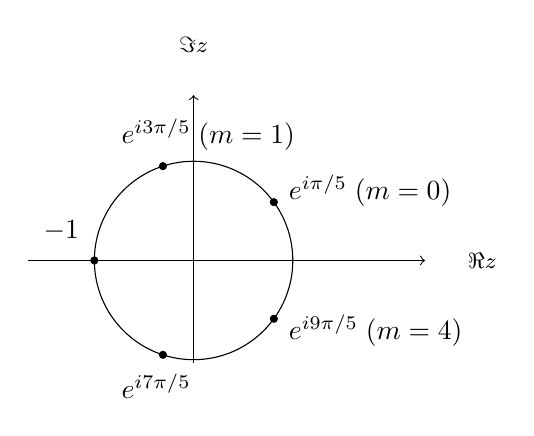
\begin{tikzpicture}[scale=.42]
\draw[->] (-5,0) -- (7,0);
\draw[->] (0,-3.1) -- (0,5);
\node[anchor=west] at (8,0) {\footnotesize $\Re z$};
\node[anchor=south] at (0,6) {\footnotesize $\Im z$};
%\foreach \x in {-5,-4,-3,-2,-1,1,2,3,4,5,6,7,8,9}
%\draw (\x,5pt) -- (\x,-5pt);
%\foreach \y in {-2,-1,1,2,3,4,5,6}
%\draw (5pt,\y) -- (-5pt,\y);
\filldraw (-3,0) circle [radius=3pt] node[anchor=south]{};

\filldraw (3*0.80901699437,3*0.587785252294) circle [radius=3pt] node[anchor=south] {};
\node[anchor=west] at (3.2*0.80901699437,3.6*0.587785252294) {$e^{i\pi/5}\; (m=0)$};
\filldraw (-3*.30901699437,3*0.95105651629) circle [radius=3pt] node[anchor=east] {};
\node[anchor=west] at (-8*.30901699437,4*0.95105651629) {$e^{i3\pi/5}\;(m=1)$};
\node[anchor=south] at (-4,.3) {$-1$};
\filldraw (-3*.30901699437,-3*0.95105651629) circle [radius=3pt] node[anchor=east] {};
\node[anchor=west] at (-8*.30901699437,-4*0.95105651629) {$e^{i7\pi/5}$};
\filldraw (3*0.80901699437,-3*0.587785252294) circle [radius=3pt] node[anchor=south] {};
\node[anchor=west] at (3.2*0.80901699437,-3.6*0.587785252294) {$e^{i9\pi/5}\; (m=4)$};

%\filldraw (3,-3) circle [radius=3pt] node[anchor=north] {$A \V{e}_2$};
%\filldraw (-7,2) circle [radius=3pt] node[anchor=east] {$A \V{u}$};
%\filldraw (9,6) circle [radius=3pt] node[anchor=north] {$A \V{v}$};
%\draw[-] (0,0) to (4,5);
%\node[anchor=south] at (2,3) {\footnotesize $r$};
\draw (3,0) arc (0:360:3);
%\node[anchor=south] at (3.3,1.1) {\footnotesize $\theta$};
%\draw[->,shorten <=4pt,shorten >=4pt] (0,1) to[bend right=30] (3,-3);
%\draw[->,shorten <=4pt,shorten >=4pt] (-1,-2) to[bend right=20] (-7,2);
%\draw[->,shorten <=4pt,shorten >=4pt] (3,2) to[bend left=20] (9,6);
\end{tikzpicture}
\\
{\small \textit{Femterøttene til -1}}
\end{center}
Merk hvordan røttene sprer seg jevnt ut på en sirkel om origo. 
Merk også at om vi lar $m> 4$ eller $m<0$, får vi røtter som allerede er listet opp.
\end{ex}

\section*{Går alt dette greit?}
Dette har vært et litt kjapt kapittel. 
Vi har jo ikke vist noe som helst, bare definert komplekse tall, sagt at $i$ oppfører seg som tallene vi kjenner fra før, 
og slengt ut en masse regneregler uten å argumentere for at dette går greit, 
eller at det i det hele tatt finnes et tallsystem der likningen
\[
x^2+1
\]
har en løsning. 

Konstruksjonen av de reelle tallene $\R$ fra de rasjonale tallene $\Q$ er komplisert nok til at selv matematikkstudenter ikke blir plaget nevneverdig med det. 
Den formelle konstruksjonen av $\C$ fra $\R$ er ikke på langt nær så komplisert, 
men man trenger fremdeles noen konsepter som ligger noe utenfor det vi kan gjøre i dette kurset.
En måte å gjøre dette på, er indikert på slutten introduksjonskapitlet. 

De reelle tallene er et eksempel på en \emph{ordnet} kropp med addisjon og multiplikasjon. 
Det at de er ordnet, betyr at man alltid kan avgjøre hvilket av to reelle tall som er størst, 
og kropp betyr at de tilfredsstiller noen aksiomer som vi ikke skal gå gjennom.

De komplekse tallene er et eksempel på en kropp som ikke er ordnet, 
siden man ikke kan si om et komplekst tall er større enn et annet, 
akkurat som vi ikke i $\R^2$ kan si at en vektor er større enn en annen. 
Du kan si at en vektor er lengre enn en annen, men det er ikke noen ordning, 
for to forskjellige vektorer kan være like lange. 
To reelle tall er like store kun dersom de er identiske.

\section*{Lineære ligninger med komplekse tall}

Et lineært likningssystem med komplekse koeffisienter og løsning, 
kan løses med gausseliminasjon på samme måte som i det reelle tilfellet.
Vi tar to eksempler.

\begin{ex}
Vi løser likningssystemet
\begin{align*}
(1-i) z + 3w   &= 2-3i \\
i z + (1+2i) w &= 1
\end{align*}
som har totalmatrise
\[
\begin{amatrix}{2}
1-i & 3 & 2-3i \\ i &1+2i & 1
\end{amatrix}.
\]
Vi ønsker å kvitte oss med $i$-en til venstre i den andre raden. 
Den første raden ganget  med $\frac{i}{1-i}$ er
\[
\begin{amatrix}{2}
i & \frac{3i}{1-i} & \frac{3+2i}{1-i} 
\end{amatrix}.
\]
Vi trekker dette fra den andre raden og erstatter den andre raden med resultatet:
\[
\begin{amatrix}{2}
1-i & 3 & 2-3i \\ 0 &1+2i -\frac{3i}{1-i} & 1-\frac{3+2i}{1-i} 
\end{amatrix}.
\]
Jeg tror vi ganger den andre raden med $1-i$ for å rydde litt:
\[
\begin{amatrix}{2}
1-i & 3 & 2-3i \\ 0 &3 -2i  & -2-3i
\end{amatrix}
\]
Vi er nå klare for å beregne $w$ og $z$:
\begin{align*}
w&=\frac{-2-3i}{3-2i}=\frac{-2-3i}{3-2i}\cdot \frac{3+2i}{3+2i}=-i \\
z&=\frac{2-3i-3(-i)}{1-i}=1+i \qedhere
\end{align*}
\end{ex}

\begin{ex}
Vi ser på systemet
\begin{align*}
	3x + y - 2z &= -1+i \\
	  x - iy     \quad\quad\;    &= 0
\end{align*}
Vi bytter rekkefølge på ligningene, slik at 
den utvidede matrisen til systemet blir:
\[
\left[
\begin{array}{ccc|c}
  1 & -i & 0 & 0 \\
  3 & 1 & -2 & -1+i
\end{array}
\right]
\]
Vi legger til $-3$ ganger første rad til andre rad og får den radekvivalente matrisen
\[
\left[
\begin{array}{ccc|c}
  1 & -i & 0 & 0 \\
  0 & 1+3i & -2 & -1+i
\end{array}
\right]
\]
Så skalerer vi andre rad ved å gange med $\frac{1-3i}{10}$ og får den radekvivalente matrisen
\[
\left[
\begin{array}{ccc|c}
  1 & -i & 0 & 0 \\
  0 & 1 & \frac{-1+3i}{5} & \frac{1+2i}{5}
\end{array}
\right]
\]
Så tar vi $i$ ganger andre rad og legger til første rad, og får matrisen på redusert trappeform
\[
\left[
\begin{array}{ccc|c}
  1 & 0 & \frac{-3-i}{5} & \frac{-2+i}{5} \\
  0 & 1 & \frac{-1+3i}{5} & \frac{1+2i}{5}
\end{array}
\right]
\]
Vi lar $z=t$ være fri variabel, og får da at generell løsning blir
\[
\vvv{x}{y}{z} = \vvv{\frac{-2+i}{5}}{\frac{1+2i}{5}}{0} + t \vvv{\frac{3+i}{5}}{\frac{1-3i}{5}}{1} \qedhere
\]
\end{ex} 


\kapittelslutt
